%%%%%%%%%%%%%%%%%%%%%%%%%%%%%%%%%%%%%%%%%%%%%%%%%%%%%%%%%%%%%%%%%%%%
% ARCA poster -- 610mm (W) x 910mm (H)
% Built for the ICML 2026 DEMO workshop demo.
% Self-contained: only uses packages shipped with TeXLive basic.
% Compile: pdflatex poster.tex   then rasterize the PDF to PNG.
%%%%%%%%%%%%%%%%%%%%%%%%%%%%%%%%%%%%%%%%%%%%%%%%%%%%%%%%%%%%%%%%%%%%
\documentclass{article}

\usepackage[paperwidth=610mm,paperheight=910mm,margin=26mm]{geometry}
\usepackage{lmodern}
\usepackage[T1]{fontenc}
\usepackage[utf8]{inputenc}
\renewcommand{\familydefault}{\sfdefault}
\usepackage{amsmath}
\usepackage{amssymb}
\usepackage{booktabs}
\usepackage{array}
\usepackage[table]{xcolor}
\usepackage{multicol}
\usepackage{tikz}
\usepackage{graphicx}

\pagestyle{empty}
\setlength{\parindent}{0pt}
\newlength{\colw}

%---------------------------------------------------------------- colours
\definecolor{primary}{RGB}{17,62,103}
\definecolor{primaryd}{RGB}{11,42,72}
\definecolor{accent}{RGB}{214,104,24}
\definecolor{accentl}{RGB}{250,233,217}
\definecolor{boxbg}{RGB}{243,246,250}
\definecolor{bandbg}{RGB}{226,237,228}
\definecolor{ink}{RGB}{30,35,42}
\color{ink}

%---------------------------------------------------------------- fonts
\newcommand{\headerfont}{\fontsize{29}{35}\selectfont\bfseries}
\newcommand{\bodyfont}{\fontsize{20}{27}\selectfont}
\newcommand{\tabfont}{\fontsize{19}{25}\selectfont}

%---------------------------------------------------------------- tight bullet list
\newenvironment{pts}
  {\begin{list}{\textcolor{accent}{\textbf{\textbullet}}}
     {\setlength{\leftmargin}{1.5em}\setlength{\labelsep}{0.5em}
      \setlength{\itemsep}{6pt}\setlength{\parsep}{0pt}\setlength{\topsep}{3pt}}}
  {\end{list}}

%---------------------------------------------------------------- block macros
\newcommand{\blockinner}[3]{%
  \begin{minipage}{#1}
    {\setlength{\fboxsep}{10pt}%
     \noindent\colorbox{primary}{\parbox{\dimexpr#1-2\fboxsep\relax}{%
        \strut\headerfont\textcolor{white}{#2}\strut}}}\par\vskip 1.5pt
    {\setlength{\fboxsep}{12pt}%
     \noindent\colorbox{boxbg}{\parbox{\dimexpr#1-2\fboxsep\relax}{%
        \bodyfont #3}}}
  \end{minipage}}

% column block (flows inside multicols)
\newcommand{\block}[2]{\par\noindent\blockinner{\linewidth}{#1}{#2}\par\vspace{16pt}}

%---------------------------------------------------------------- token-weight panel
% \wpanel{x-offset}{title}{bar color}{caption}{index/weight/token list}
\newcommand{\wpanel}[5]{%
  \begin{scope}[shift={(#1,0)}]
    \fill[boxbg,rounded corners=5pt] (-0.45,-2.4) rectangle (14.7,7.0);
    \node[anchor=north,font=\bfseries\fontsize{21}{24}\selectfont,text=primary]
      at (7.1,6.85) {#2};
    \draw[primaryd!55,dashed,line width=0.9pt] (0,2.25) -- (14.25,2.25);
    \draw[ink!60,line width=1.1pt] (0,0) -- (14.25,0);
    \foreach \j/\w/\tok in {#5}{
      \pgfmathsetmacro{\xc}{0.9 + \j*1.74}
      \fill[#3,rounded corners=2pt] ({\xc-0.52},0) rectangle ({\xc+0.52},{\w*5.0});
      \node[anchor=north,font=\ttfamily\fontsize{15}{17}\selectfont,text=ink]
        at (\xc,-0.2) {\tok};
    }
    \node[anchor=north,font=\itshape\fontsize{16}{19}\selectfont,text=ink]
      at (7.1,-1.55) {#4};
  \end{scope}}

\begin{document}

%================================================================ TITLE BANNER
\noindent
{\setlength{\fboxsep}{20pt}%
\colorbox{primary}{\parbox{\dimexpr\textwidth-2\fboxsep\relax}{%
  \centering
  {\fontsize{62}{70}\selectfont\bfseries\textcolor{white}{ARCA: Adapter-Residual Credit Assignment}}\\[10pt]
  {\fontsize{40}{48}\selectfont\bfseries\textcolor{accentl}{When Token Signals Degenerate}}\\[18pt]
  {\fontsize{30}{38}\selectfont\textcolor{white}{Rodney Lafuente-Mercado \quad$\cdot$\quad Scale AI \quad$\cdot$\quad rodney.lafuente@scale.com}}\\[10pt]
  {\fontsize{22}{28}\selectfont\textcolor{white!82}{DEMO 2026 \;$\cdot$\; ICML Workshop on Decision-Making from Offline Datasets to Online Adaptation \;$\cdot$\; \texttt{github.com/rodlaf/tokenweighting}}}%
}}}

\vspace{16pt}

%================================================================ TL;DR STRIP
\noindent
{\setlength{\fboxsep}{16pt}%
\fcolorbox{accent}{accentl}{\parbox{\dimexpr\textwidth-2\fboxsep-2\fboxrule\relax}{%
  \fontsize{24}{32}\selectfont
  \textcolor{accent}{\textbf{TL;DR.}}\;
  Practical LLM-RL runs on \textbf{LoRA}, but standard token-credit signals
  (surprisal, entropy reduction, policy divergence) \textbf{degenerate} under
  low-rank adaptation. They collapse either to uniform broadcast or to spurious
  sparsity. \textbf{ARCA} instead reads salience straight from the adapter's own
  hidden-state residual $\lVert h^{\text{adapted}}_t - h^{\text{base}}_t\rVert_2$,
  with no critic, no reward model, and no trees. It keeps credit in a useful
  middle regime and stays competitive at matched parameters.%
}}}

\vspace{16pt}

%================================================================ CONCEPT GRAPHIC (full width)
\noindent\blockinner{\textwidth}{How ARCA assigns token credit}{%
Each token's pull on the gradient in $g = A\sum_t w_t\,\nabla\!\log\pi_\theta(y_t)$
is its weight $w_t$ (bar height below). ARCA sets $w_t=\lVert h^{\text{adapted}}_t - h^{\text{base}}_t\rVert_2$,
so the tokens the adapter changes most get the most credit. The dashed line marks the uniform weight.
\par\vspace{10pt}
\centering
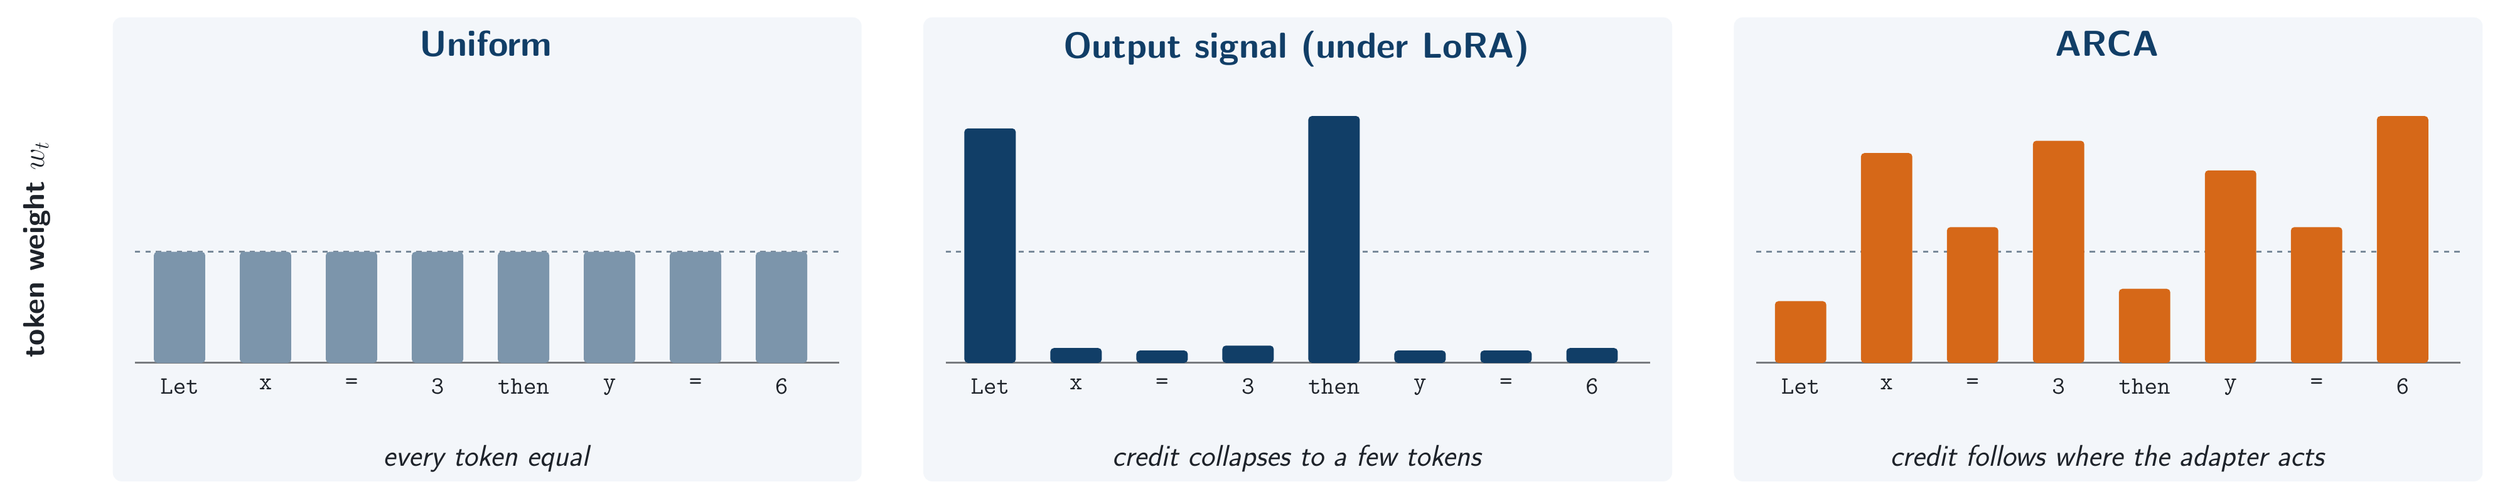
\begin{tikzpicture}[x=1cm,y=1cm]
  % y-axis label
  \node[rotate=90,anchor=south,font=\bfseries\fontsize{17}{19}\selectfont,text=ink]
    at (-1.6,2.3) {token weight $w_t$};
  % three panels
  \wpanel{0}{Uniform}{primary!55}{every token equal}%
    {0/.45/Let,1/.45/x,2/.45/{=},3/.45/3,4/.45/then,5/.45/y,6/.45/{=},7/.45/6}
  \wpanel{16.4}{Output signal (under LoRA)}{primary}{credit collapses to a few tokens}%
    {0/.95/Let,1/.06/x,2/.05/{=},3/.07/3,4/1.0/then,5/.05/y,6/.05/{=},7/.06/6}
  \wpanel{32.8}{ARCA}{accent}{credit follows where the adapter acts}%
    {0/.25/Let,1/.85/x,2/.55/{=},3/.9/3,4/.3/then,5/.78/y,6/.55/{=},7/1.0/6}
\end{tikzpicture}}

\vspace{20pt}

%================================================================ BODY (3 columns)
\setlength{\columnsep}{22pt}
\begin{multicols}{3}
\raggedcolumns

\block{1.\; The Problem}{%
\begin{pts}
\item RL drives LLM post-training, but \textbf{credit assignment} is hard:
trajectories are long and the reward is a single sparse outcome scalar.
\item Intrinsic token weighting reads per-token salience off the model's own
output distribution (surprisal, entropy, divergence).
\item Yet \textbf{most real LLM-RL pipelines use LoRA} for memory and compute.
\item These threads are studied apart. We show their \textbf{interaction} is the
real issue.
\end{pts}}

\block{2.\; Failure Mode: Signal Degeneration under LoRA}{%
LoRA confines the policy $\pi_\theta$ to a low-rank neighborhood of the
reference $\pi_{\text{ref}}$ (an implicit KL bound), so the per-token output
differences these signals measure are
\[
-\log\pi_\theta(y_t)= -\log\pi_{\text{ref}}(y_t)+O(\lVert\Delta h_t\rVert),
\]
\textbf{dominated by the base model}, not the adapter. After within-trajectory
normalization the weights degenerate:
\begin{pts}
\item \textbf{Uniform broadcast}: Gini $G(w)\!\approx\!0$ when the $\varepsilon$ floor dominates.
\item \textbf{Spurious sparsity}: $G(w)\!\approx\!1$ with a tiny effective support $\mathrm{EffN}/T$.
\end{pts}
\vspace{4pt}
Either way the weights stop tracking where the adapter acts. Read it off
directly with \textbf{Gini} $G(w)$ and the \textbf{effective-token ratio}
$\mathrm{EffN}(w)/T=1/\!\big(T\textstyle\sum_t w_t^2\big)$.}

\block{3.\; ARCA}{%
Measure salience where LoRA actually acts, in the adapter's own contribution to
the forward pass:
\[
\boxed{\;\alpha_t^{\mathrm{ARCA}}=\big\lVert h^{\text{adapted}}_t-h^{\text{base}}_t\big\rVert_2\;}
\]
then normalize within each trajectory to weights $w_t^{\mathrm{ARCA}}$.
\begin{pts}
\item One extra no-grad forward pass with \texttt{model.disable\_adapter()}, the
same call already used for the KL term or divergence weighting. No new
infrastructure.
\item Weights are \textbf{detached}: no second-order terms, cost close to a
critic-free policy gradient.
\item No value head, no learned process reward model, no search trees.
\end{pts}}

\block{4.\; Why ARCA Avoids Collapse}{%
\begin{pts}
\item Even when $\lVert B_\ell A_\ell\rVert$ is small, the adapter input
activations $x_{\ell,t}$ stay \textbf{non-uniform across positions} (attention,
layer norm, content vs filler), so $\lVert\Delta h_t\rVert$ keeps real
position-to-position variation.
\item It reads as cheap \textbf{gradient-informed} credit: a large residual
marks positions where a policy-gradient update has the most effect.
\item With a fixed $\varepsilon$ floor, any score whose magnitude vanishes
eventually normalizes to uniform. ARCA's residual stays measurable, so its
weights remain tied to adapter activity instead of to floor numerics.
\end{pts}}

\block{5.\; Experimental Setup}{%
\begin{pts}
\item \texttt{Qwen3-1.7B-Base}, \textbf{MATH}, \textbf{GRPO}, binary exact-match reward, LoRA on attn and MLP.
\item $K\!=\!4$ completions per prompt, 100 update steps, seed 1337; eval greedy accuracy and pass@4 on 200 held-out.
\item \textbf{7 runs}: uniform, surprisal, entropy reduction, policy divergence at $r\!=\!64$; ARCA at $r\!\in\!\{4,16,64\}$.
\item AdamW at lr $5\times10^{-6}$, 10-step warmup then cosine decay, batch size 2 with 4-step gradient accumulation, prompt and generation length capped at 512, temperature 1.0, top-$p$ 0.95.
\item Same rollout groups, optimizer, schedule, and decoding across methods, so token redistribution is the only algorithmic difference. Each run fits on one H100-class GPU in a few hours.
\end{pts}}

\block{6.\; Held-out MATH Performance}{%
\centering\tabfont
\renewcommand{\arraystretch}{1.36}
\setlength{\tabcolsep}{7pt}
\begin{tabular}{l c c c c}
\toprule
\textbf{Method} & $r$ & \textbf{Greedy} & \textbf{Pass@4} & \textbf{Tr.\ rew.}\\
\midrule
Uniform           & 64 & \textbf{0.620} & 0.675 & 0.362\\
Surprisal         & 64 & 0.520 & 0.650 & 0.326\\
Entropy reduction & 64 & 0.600 & \textbf{0.700} & 0.367\\
Policy divergence & 64 & 0.565 & 0.670 & 0.351\\
\rowcolor{accentl} ARCA & 4  & 0.525 & 0.640 & 0.327\\
\rowcolor{accentl} ARCA & 16 & 0.510 & 0.655 & 0.336\\
\rowcolor{accentl} ARCA & 64 & 0.590 & 0.680 & 0.353\\
\bottomrule
\end{tabular}
\par\vspace{8pt}
\raggedright\fontsize{18}{24}\selectfont
At matched rank 64, ARCA is competitive: 3 points under uniform on greedy and
0.5 point over it on pass@4. Lower-rank ARCA trails the rank-64 baselines, which
points to a capacity effect rather than an extra-parameter effect. No single
weighting wins outright here: uniform takes greedy and entropy reduction takes
pass@4, so read this table as a compact validation, not a benchmark sweep.}

\block{7.\; The Central Result: Credit Concentration}{%
\centering\tabfont
\renewcommand{\arraystretch}{1.36}
\setlength{\tabcolsep}{9pt}
\begin{tabular}{l c c c}
\toprule
\textbf{Method} & $r$ & $G(w)$ & $\mathrm{EffN}/T$\\
\midrule
Uniform           & 64 & 0.000 & 1.000\\
Surprisal         & 64 & 0.941 & 0.052\\
Entropy reduction & 64 & 0.920 & 0.073\\
Policy divergence & 64 & 0.939 & 0.055\\
\rowcolor{accentl} ARCA & 4  & 0.353 & 0.467\\
\rowcolor{accentl} ARCA & 16 & 0.388 & 0.460\\
\rowcolor{accentl} ARCA & 64 & 0.490 & 0.334\\
\bottomrule
\end{tabular}

\vspace{14pt}
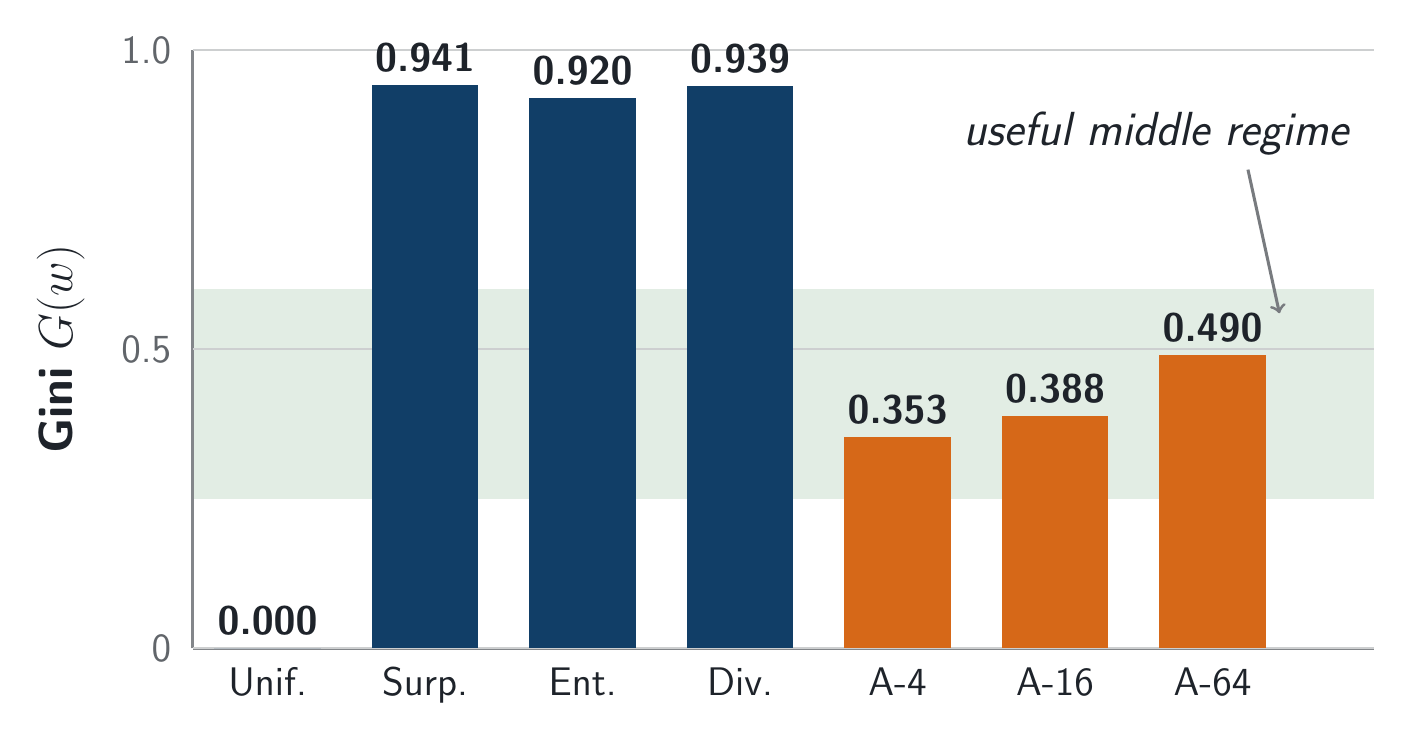
\begin{tikzpicture}[x=1cm,y=1cm]
  \def\W{15.0}
  \def\H{7.6}
  \fill[bandbg] (0,{0.25*\H}) rectangle (\W,{0.60*\H});
  \node[anchor=east,text=ink,font=\fontsize{16}{18}\selectfont\itshape]
     at ({\W-0.2},{0.86*\H}) {useful middle regime};
  \draw[->,ink!60,line width=1.1pt]
     ({\W-1.6},{0.80*\H}) -- ({\W-1.2},{0.56*\H});
  \draw[ink!55,line width=1pt] (0,0) -- (\W,0);
  \draw[ink!55,line width=1pt] (0,0) -- (0,\H);
  \foreach \g in {0,0.5,1.0}{
     \draw[ink!22,line width=0.7pt] (0,{\g*\H}) -- (\W,{\g*\H});
     \node[anchor=east,text=ink!70,font=\fontsize{15}{17}\selectfont] at (-0.15,{\g*\H}) {\g};
  }
  \node[rotate=90,anchor=south,text=ink,font=\fontsize{17}{19}\selectfont\bfseries]
     at (-1.25,{0.5*\H}) {Gini $G(w)$};
  \def\bw{1.35}
  \foreach \i/\v/\lab/\col in {%
     0/0.000/Unif./primary,
     1/0.941/Surp./primary,
     2/0.920/Ent./primary,
     3/0.939/Div./primary,
     4/0.353/A-4/accent,
     5/0.388/A-16/accent,
     6/0.490/A-64/accent}{
     \pgfmathsetmacro{\xc}{0.95 + \i*2.0}
     \fill[\col] ({\xc-\bw/2},0) rectangle ({\xc+\bw/2},{\v*\H});
     \node[anchor=south,text=ink,font=\fontsize{14}{16}\selectfont\bfseries]
        at (\xc,{\v*\H+0.05}) {\v};
     \node[anchor=north,text=ink,font=\fontsize{15}{17}\selectfont]
        at (\xc,-0.12) {\lab};
  }
\end{tikzpicture}
\par\vspace{6pt}
\raggedright\fontsize{18}{24}\selectfont
The baselines sit at the extremes ($G\!\approx\!0$ or $\approx\!0.94$). ARCA
lands in the predicted middle: non-uniform, but not collapsed onto a handful of
tokens. Output signals ask where the model is uncertain; ARCA asks where the
adapter acts.}

\block{8.\; Contributions}{%
\begin{pts}
\item We formalize a PEFT-specific failure mode: under LoRA, token salience
collapses to uniform broadcast or spurious sparsity.
\item We introduce \textbf{ARCA}, an adapter-residual credit rule whose weights
stay non-degenerate when the adapter varies by position.
\item We validate it with concentration diagnostics and a matched
MATH/Qwen3-1.7B sweep.
\end{pts}}

\block{9.\; Takeaways}{%
\begin{pts}
\item Token-level credit assignment and PEFT are \textbf{coupled}, not orthogonal.
\item Under LoRA, output-distribution signals degenerate, so a null result for
``elaborate weighting vs uniform'' can be a LoRA artifact.
\item \textbf{ARCA} gives an adaptation-aware, lightweight, non-degenerate credit
signal that stays competitive at matched parameters.
\end{pts}}

\end{multicols}

\end{document}
